\documentclass{article} 
\UseRawInputEncoding
\usepackage[utf8]{inputenc}
\usepackage[T1]{fontenc}
\usepackage{selinput}
\usepackage[spanish]{babel}
\usepackage{hyphenat}
\usepackage{graphicx} 
\usepackage{subcaption}
\usepackage{hyperref}
\usepackage{listings}
\usepackage{xcolor}
\usepackage{float}
\usepackage[a4paper, total={6in, 9in}]{geometry}
\SelectInputMappings{%
  eacute={é},
}

\definecolor{codegreen}{rgb}{0,0.6,0}
\definecolor{codegray}{rgb}{0.5,0.5,0.5}
\definecolor{codepurple}{rgb}{0.58,0,0.82}
\definecolor{backcolour}{rgb}{0.95,0.95,0.92}

\lstdefinestyle{mystyle}{
    backgroundcolor=\color{backcolour},
    commentstyle=\color{codegreen},
    keywordstyle=\color{blue},
    numberstyle=\tiny\color{codegray},
    stringstyle=\color{codepurple},
    basicstyle=\ttfamily\footnotesize,
    breakatwhitespace=false,
    breaklines=true,
    captionpos=b,
    keepspaces=true,
    numbers=left,
    numbersep=5pt,
    showspaces=false,
    showstringspaces=false,
    showtabs=false,
    tabsize=2
}

\lstdefinelanguage{CSS}{
  keywords={color,background-image:,margin,padding,font,weight,display,position,top,left,right,bottom,list,style,border,size,white,space,min,width, transition:, transform:, transition-property, transition-duration, transition-timing-function},	
  sensitive=true,
  morecomment=[l]{//},
  morecomment=[s]{/*}{*/},
  morestring=[b]',
  morestring=[b]",
  alsoletter={:},
  alsodigit={-}
}
\lstset{style=mystyle}
\title{Carpeta de Campo BIAS}

\date{}

\begin{document}

\begin{figure}
    \centering
    
\includegraphics[width=0.95\linewidth]{Imagenes//BIAS/LogoBIASbn.png}
\end{figure}

\maketitle

\vspace{1cm} 

\textbf{Integrantes del Proyecto:} 

\begin{itemize}
    \item Adell, Nicolas Fabian
    \item De Blasi, Luca
    \item Diaz Melion, Danilo Sebastian
    \item Gil Soria, Ian Lucas
    \item Montenegro, Luciano Nahuel
    \item Sojka, Santiago Alejandro
\end{itemize}

\newpage


\subsection{Adell, Nicolás Fabián}

\begin{figure}[H]
    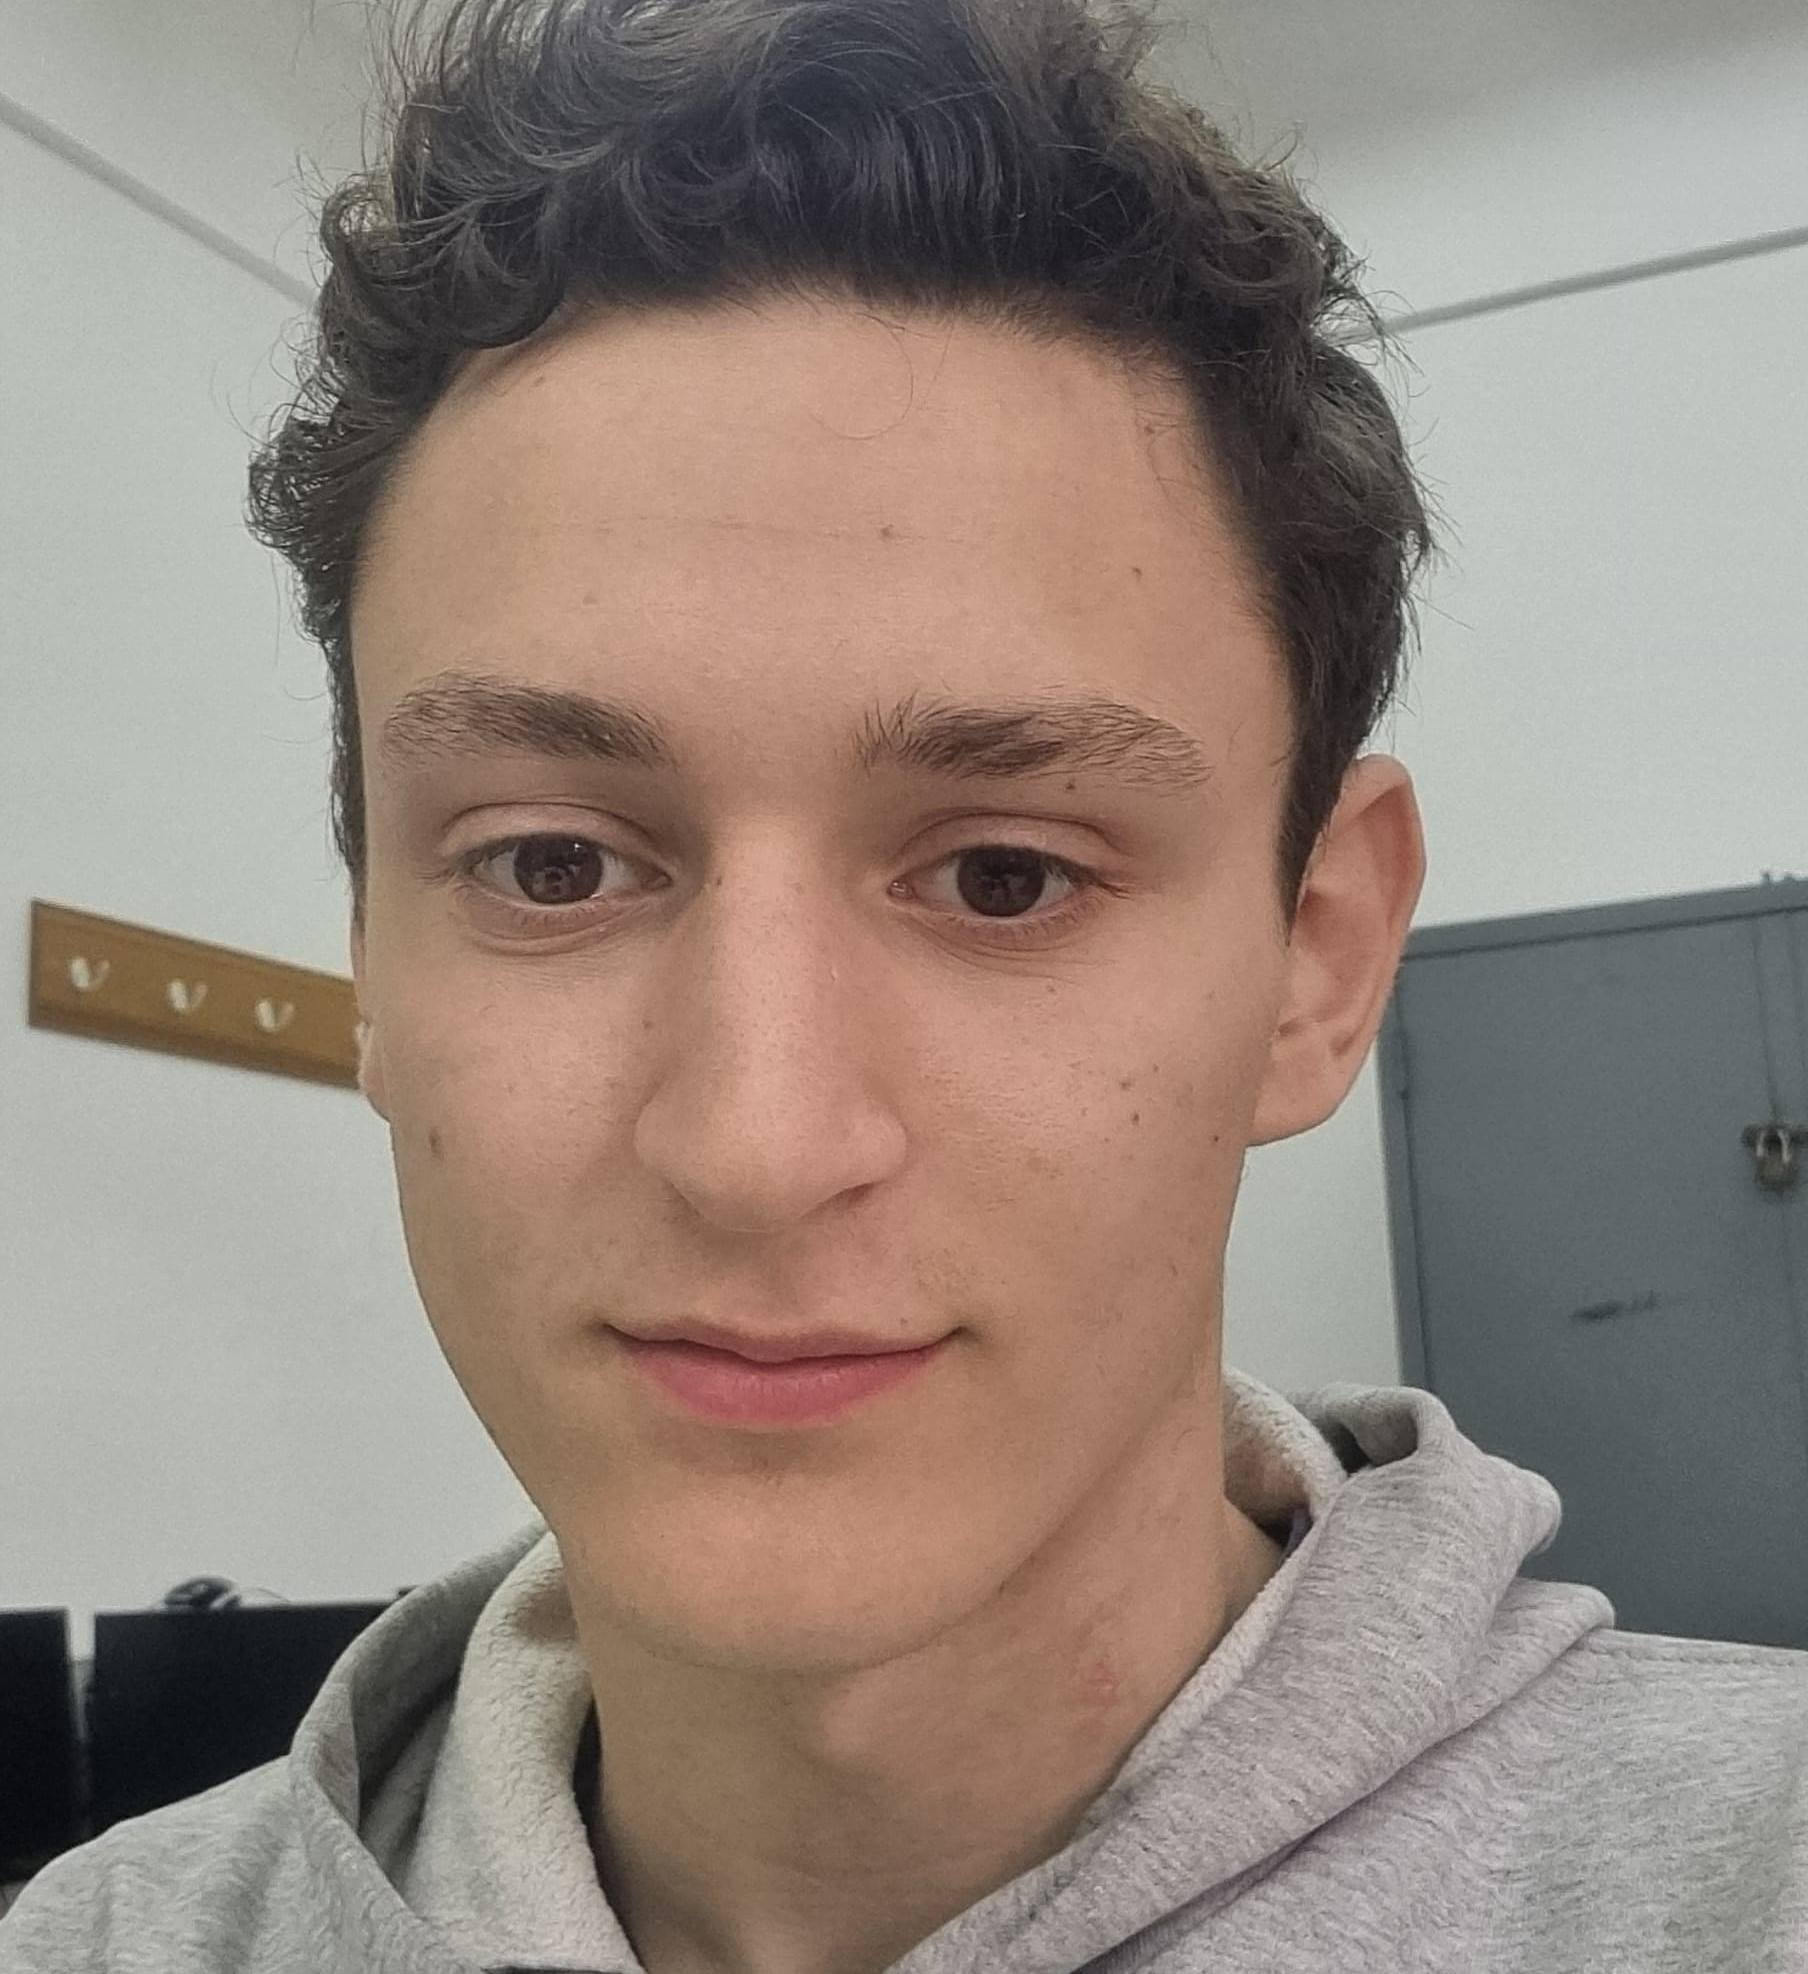
\includegraphics[width=0.3\linewidth]{Imagenes//BIAS/Fabi.jpg}
\end{figure}

\subsection{De Blasi, Luca}

\begin{figure}[H]
    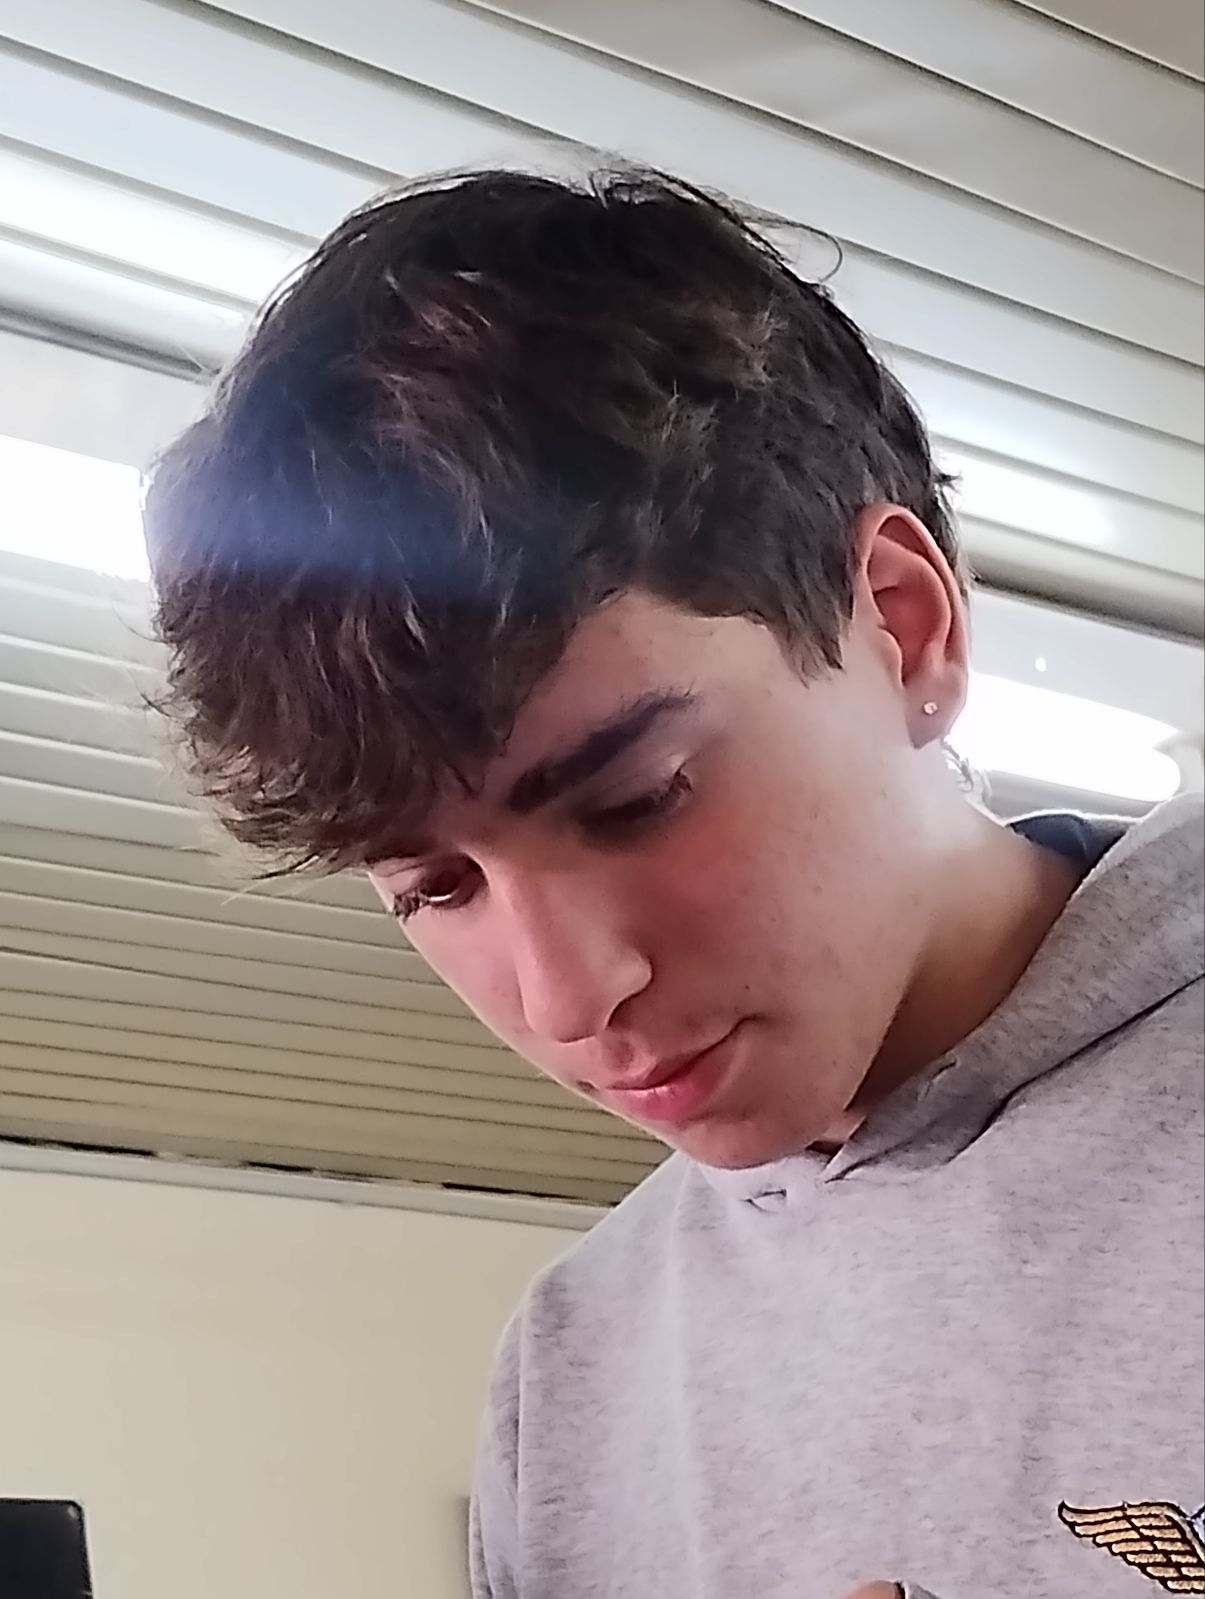
\includegraphics[width=0.3\linewidth]{Imagenes//BIAS/pela.jpg}
\end{figure}

\subsection{Diaz Melión, Danilo Sebastián}

\begin{figure}[H]
    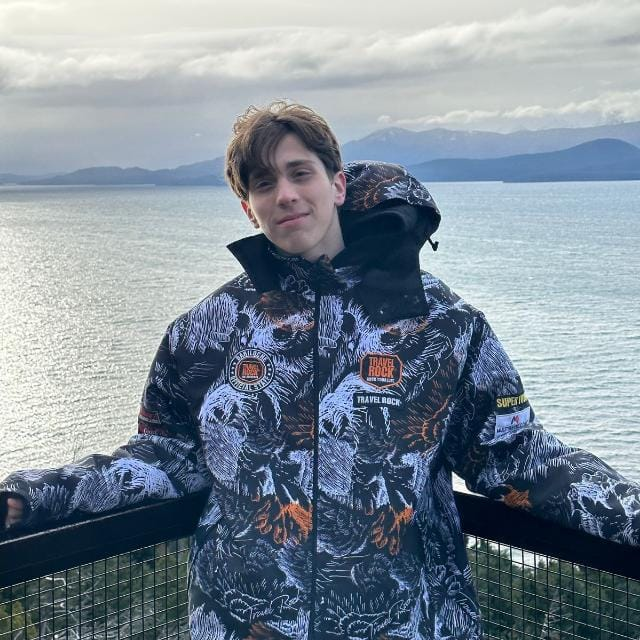
\includegraphics[width=0.3\linewidth]{Imagenes//BIAS/Dani.jpg}
\end{figure}

\subsection{Gil Soria, Ian Lucas}

\begin{figure}[H]
    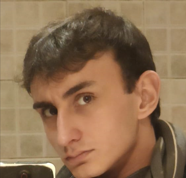
\includegraphics[width=0.3\linewidth]{Imagenes//BIAS/Soria2.png}
\end{figure}

\subsection{Montenegro, Luciano Nahuel}

\begin{figure}[H]
    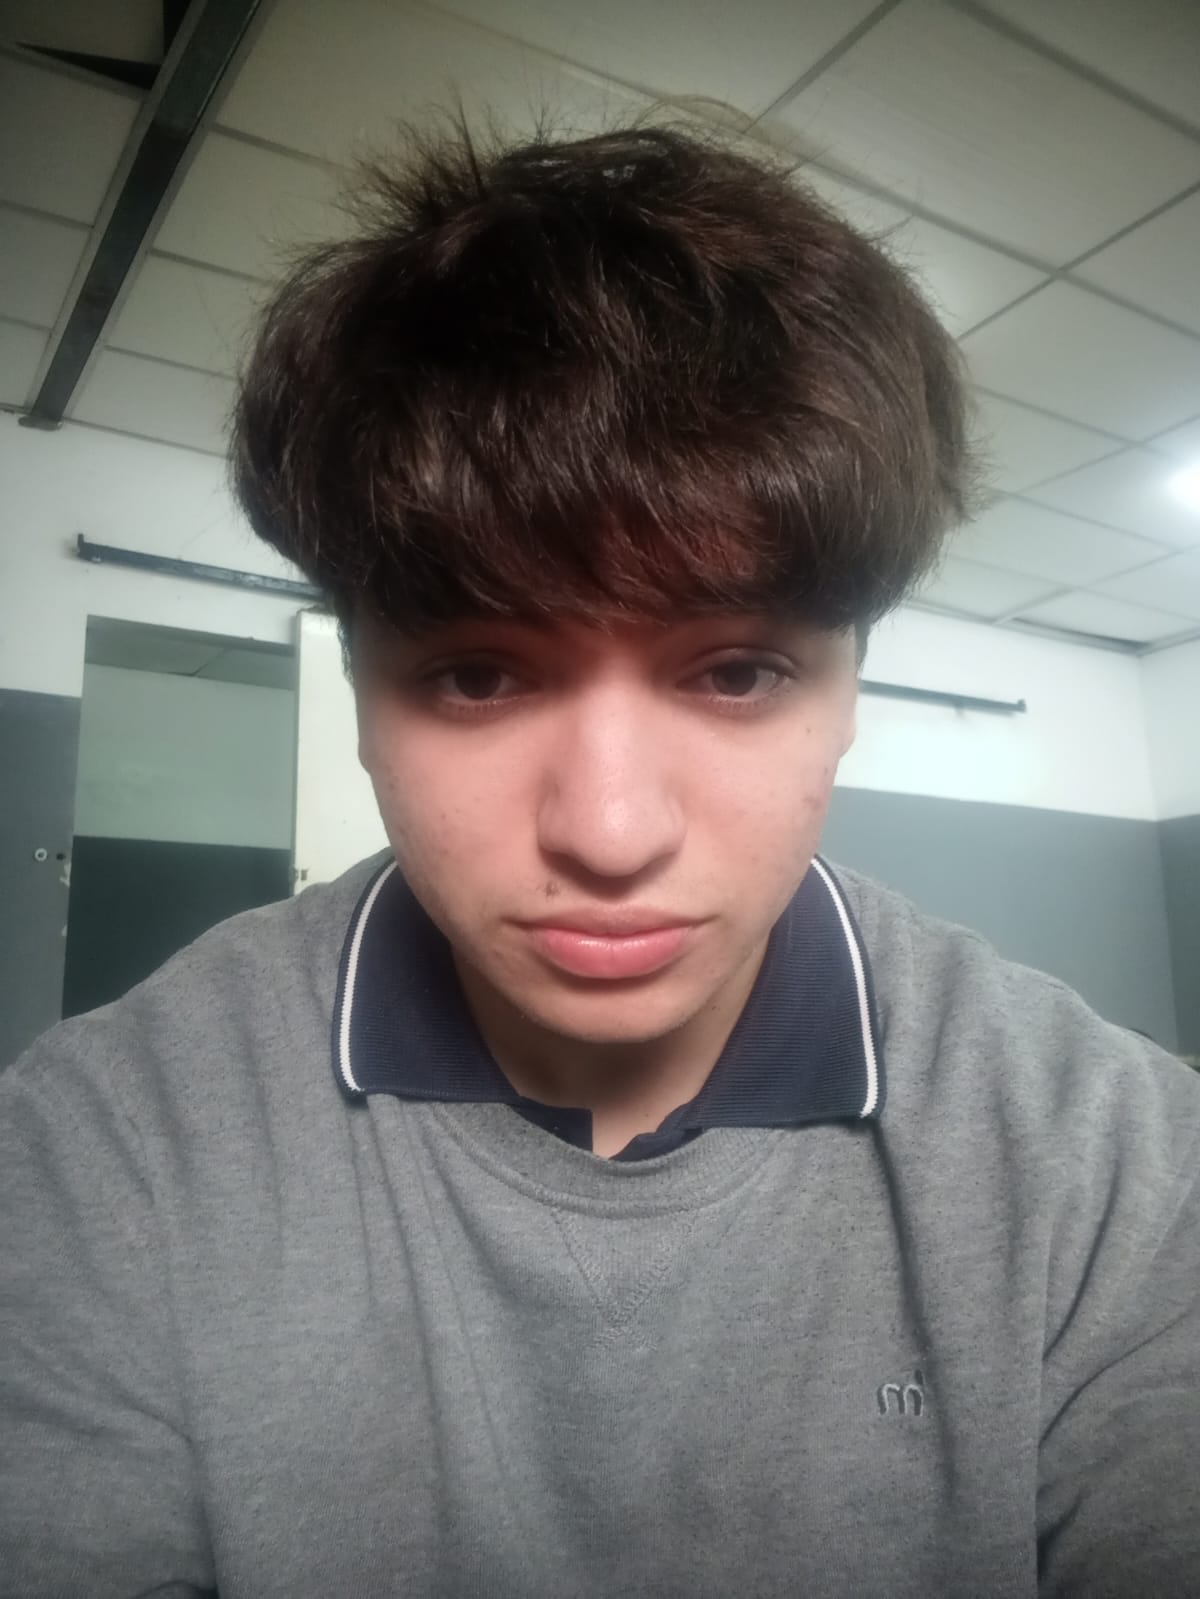
\includegraphics[width=0.3\linewidth]{Imagenes//BIAS/Lucho.jpg}
\end{figure}

\subsection{Sojka, Santiago Alejandro}

\begin{figure}[H]
    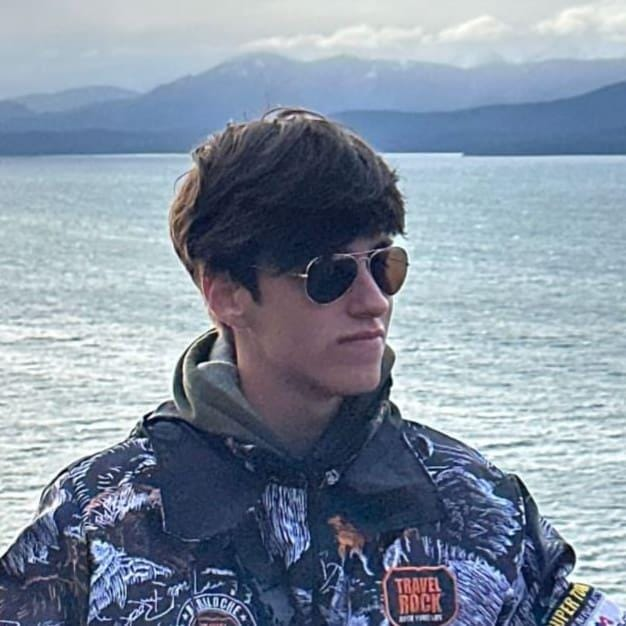
\includegraphics[width=0.3\linewidth]{Imagenes//BIAS/Sojka2.jpg}
\end{figure}




\newpage

\section{Marzo de 2024}

Inicio de anteproyecto e investigación sobre la utilización de MATLAB, Python y cómo vincular el Neurosky Mindwave Mobile 2 a una computadora o celular. Decisión de elección de microcontrolador y hardware a utilizar.

\begin{center}
    \href{https://theses.hal.science/tel-04011453v1/document}{https://theses.hal.science/tel-04011453v1/document}
\end{center}

Realización y testeo del código para poder mover la silla de ruedas mediante un joystick.
Investigación sobre los posibles materiales a utilizar en el proyecto ya existentes en la escuela. Hemos visto las posibles sillas de ruedas a utilizar en el proyecto.
Investigación del sensor ultrasónico a utilizar en el proyecto.

Hemos empezado a realizar la programación de los motores y la programación del ultrasonido y se han probado en protoboard, probando que funcionan. También se han hecho ciertas modificaciones al anteproyecto, y se ha empezado a hacer el diagrama temporal. 

\begin{figure}[H]
    \centering
    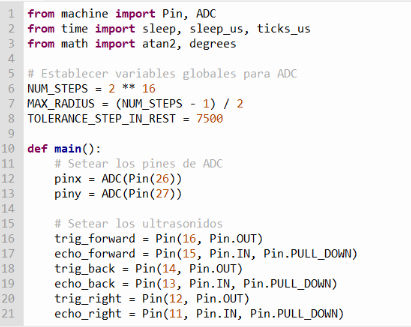
\includegraphics[width=0.95\linewidth]{Imagenes//Marzo/ProgramacionMotores.png}
\end{figure}

\newpage

Hemos hecho el logo del proyecto, hemos encontrado las baterías necesarias para poder mover la silla de ruedas, discutimos, tanto entre nosotros como con otros profesores, sobre la utilización de 1 o 2 motores, discutimos sobre los drivers y el puente H.

\begin{figure}[H]
    \centering
    
\includegraphics[width=0.75\linewidth]{Imagenes//Marzo/LogoBIAS.png}
\end{figure}

En el día de la fecha hemos creado la cuenta  de la red social instagram junto al mail mismo del proyecto.

\begin{figure}[H]
    \centering
    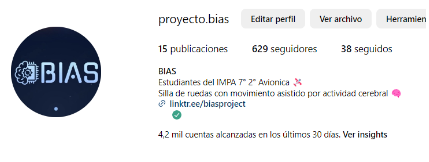
\includegraphics[width=0.75\linewidth]{Imagenes//Marzo/InstagramBias.png}
\end{figure}


Hemos realizado el esquemático junto al diseño del pcb del sistema de emergencias, por lo que quedaría imprimirlo y ya ir armando la placa.

\begin{figure}[H]
    \centering
    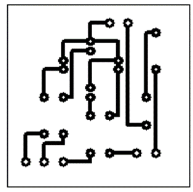
\includegraphics[width=0.45\linewidth]{Imagenes//Marzo/SistemadeEmergencias.png}
\end{figure}

\newpage

Investigamos la datasheet del driver del motor, empezamos a investigar el circuito interno y las posibilidades a la hora de manejar el motor.

\begin{figure}[H]
    \centering
    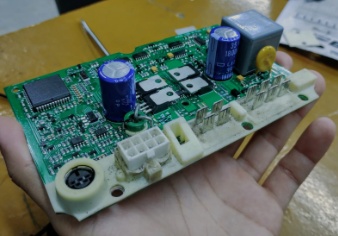
\includegraphics[width=0.65\linewidth]{Imagenes//Marzo/DriverFoto.png}
\end{figure}

Empezamos a desarrollar el programa para conectar el Neurosky a un módulo HC-05.

\begin{figure}[H]
    \centering
    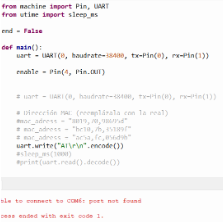
\includegraphics[width=0.65\linewidth]{Imagenes//Marzo/ProgramaNeurosky.png}
\end{figure}

\newpage

\begin{center}
    \section{Abril de 2024}
\end{center}

Hemos empezado a organizarnos con la plataforma trello para tener buena percepción sobre las tareas a realizar.

\begin{figure}[H]
    \centering
    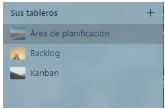
\includegraphics[width=0.6\linewidth]{Imagenes//Abril/Trello.png}
\end{figure}

Estuvimos buscando la forma de conectar el Neurosky a la computadora a través de bluetooth, y terminamos optando por seguir con el HC-05, ya que no se conecta directamente y las versiones no son compatibles.



\begin{figure}[H]
    \centering
    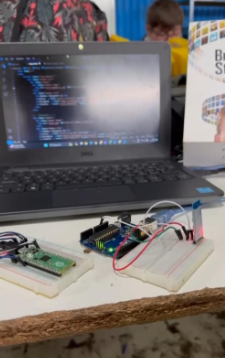
\includegraphics[width=0.45\linewidth]{Imagenes//Abril/ProgramacionNeurosky.png}
\end{figure}

\newpage

Hicimos las imágenes que vamos a publicar al Instagram a la hora de que verifiquen el LinkedIn, seguimos desarrollando el programa para usar el módulo bluetooth (HC-05), empezamos a hacer un plano de la silla de ruedas para hacer las modificaciones de la estructura que tengamos que hacer.

\begin{figure}[H]
    \centering
    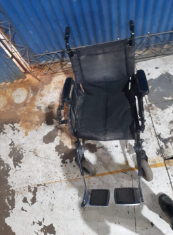
\includegraphics[width=0.45\linewidth]{Imagenes//Abril/SilladeRuedas.png}
\end{figure}

Se consiguió con éxito poder establecer la conexión Bluetooth del HC05 a una computadora 

\begin{figure}[H]
    \centering
    \includegraphics[width=0.5\linewidth]{Imagenes//Abril/HC05.png}
\end{figure}

\newpage

Cargamos las baterías y empezamos a probar los motores junto al driver, investigamos sobre otras opciones para reemplazar al Neurosky, ya que no hay forma de hacerlos vincular..

\begin{figure}[H]
    \centering
    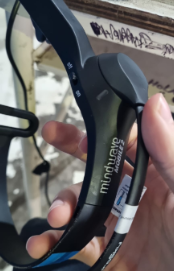
\includegraphics[width=0.25\linewidth]{Imagenes//Abril/Neurosky.png}
\end{figure}

Desarrollamos la página del proyecto, creamos el GitHub donde estará todo tipo de documento y código relacionado al proyecto y una cuenta de TikTok.

\begin{figure}[H]
    \centering
    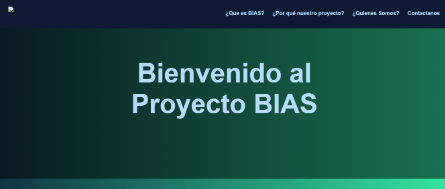
\includegraphics[width=0.65\linewidth]{Imagenes//Abril/PaginaWeb.png}
\end{figure}

Seguimos con la programación del Neurosky Mobile Mindwave 2, además de crear publicaciones para difundirnos por Instagram.

\begin{figure}[H]
    \centering
    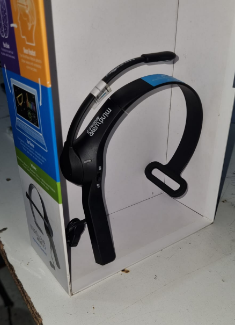
\includegraphics[width=0.35\linewidth]{Imagenes//Abril/NeuroskyCaja.png}
\end{figure}

\newpage


\begin{center}
    \section{Mayo de 2024}
\end{center}






Probamos conectar el Neurosky con Arduino pero sigue sin funcionar. Por eso buscamos otras alternativas para el EEG, ya que debido a los intentos reiterados no funciona.

\begin{figure}[H]
    \centering
    \includegraphics[width=0.3\linewidth]{Imagenes//Mayo/HC05.png}
\end{figure}



Se investiga el driver si puede funcionar y si es viable utilizarlo o hacer el propio.

\begin{figure}[H]
    \centering
    \includegraphics[width=0.85\linewidth]{Imagenes//Mayo/Servos.png}
\end{figure}

\newpage

Fuimos a la radio en Solano a hablar del proyecto. Nos contactamos con la radio FM Sur.

\begin{figure}[H]
    \centering
    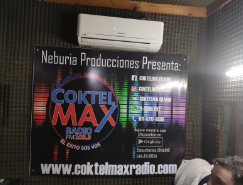
\includegraphics[width=0.5\linewidth]{Imagenes//Mayo/RadioCoktel.png}
\end{figure}


Probamos el driver y el motor originales que venían con la silla de ruedas. Se realiza un informe sobre el Driver ya que el mismo no funciona.

\begin{figure}[H]
    \centering
    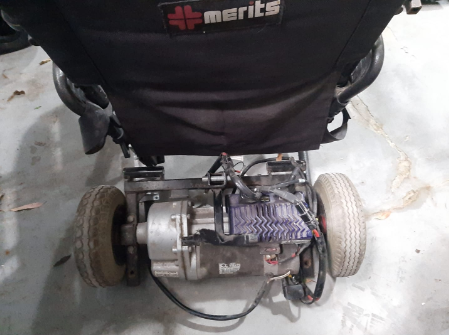
\includegraphics[width=0.55\linewidth]{Imagenes//Mayo/SillaMotor.png}
\end{figure}

Se realizó el plano de la silla de ruedas en Autocad. Se busca la forma de diseño del Driver. Nos contactamos con sponsors para darnos difusión. Organizamos el Trello.

\begin{figure}[H]
    \centering
    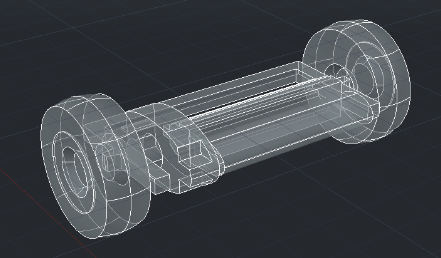
\includegraphics[width=0.55\linewidth]{Imagenes//Mayo/MotorModelo3D.png}
\end{figure}


\newpage

Tuvimos la entrevista radial en FM Sur. Se realiza el reel n.° 3. Se continúa con el plano de la silla. Se organiza el Github. Se buscan alternativas al Neurosky. 

\begin{figure}[H]
    \centering
    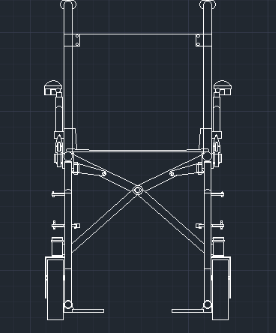
\includegraphics[width=0.55\linewidth]{Imagenes//Mayo/SillaModelo3D.png}
\end{figure}

Se realiza el diseño del driver para el motor. Finalmente se toma el Open BCI como alternativa para realizarla por nosotros mismos debido a los costes de fabricación. Para eso se busca la documentación.

\begin{figure}[H]
    \centering
    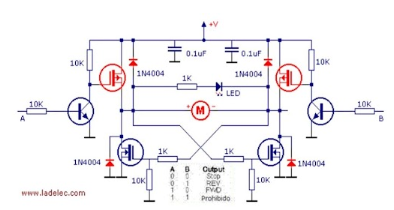
\includegraphics[width=0.85\linewidth]{Imagenes//Mayo/PuenteH.png}
\end{figure}

\newpage

Nos contactamos con ALAPA, con la Fundación Esteban Bullrich y con la política María Sotolano. Vemos la alternativa del Open BCI

\begin{figure}[H]
    \centering
    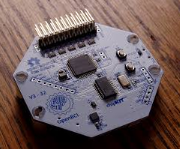
\includegraphics[width=0.45\linewidth]{Imagenes//Mayo/OpenBCI.png}
\end{figure}

Realizamos una entrevista para que Clarín haga una nota sobre nosotros.

\begin{figure}[H]
    \centering
    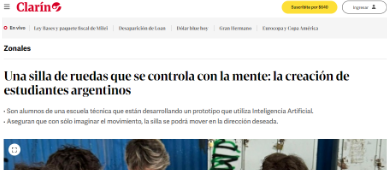
\includegraphics[width=0.75\linewidth]{Imagenes//Mayo/Clarin.png}
\end{figure}




Buscamos de un EEG de reemplazo que tenga un coste aceptable. Elegimos entre el Open BCI y otro circuito. Tomamos el ejemplo de la página siguiente: 

\begin{center}
    \href{https://www.instructables.com/DIY-EEG-and-ECG-Circuit/}{https://www.instructables.com/DIY-EEG-and-ECG-Circuit}
\end{center}

\begin{figure}[H]
    \centering
    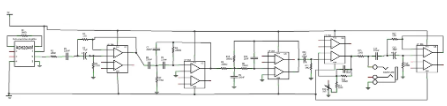
\includegraphics[width=0.85\linewidth]{Imagenes//Mayo/EEG.png}
\end{figure}

\newpage

Fuimos al Congreso a hablar con la diputada María Sotolano. Logramos asegurar el contacto con la asociación Esteban Bullrich.

\begin{figure}[H]
    \centering
    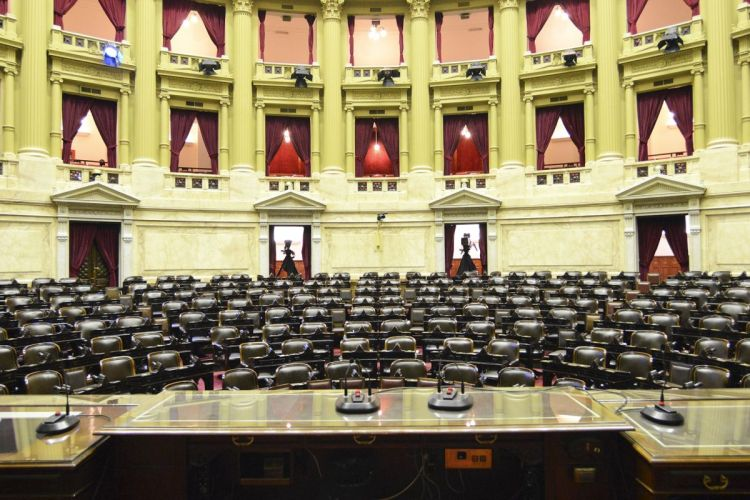
\includegraphics[width=0.75\linewidth]{Imagenes//Mayo/CamaraDiputados.jpg}
\end{figure}

TN nos entrevista, por lo que preparamos un stand para presentar en la televisión.

\begin{figure}[H]
    \centering
    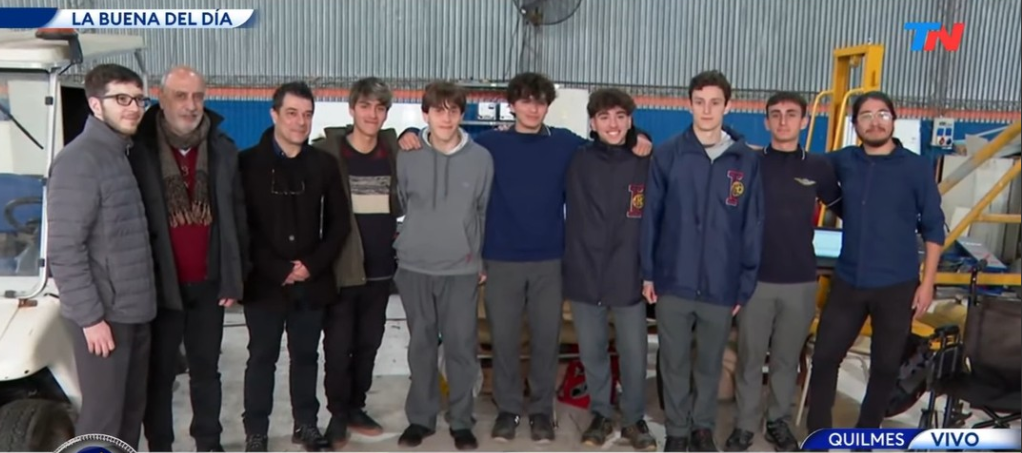
\includegraphics[width=0.95\linewidth]{Imagenes//Mayo/bias.png}
\end{figure}

\newpage


\begin{center}
    \section{Junio de 2024}
\end{center}

Damos entrevista con Radio Nacional. Se comunica con nosotros TV pública y Radio Halley. Se hace diseño en KiCad del EEG. Se empieza a programar EEG mediante transformada de Fourier. Luego se filtra la señal y se discrimina por tipo de frecuencia. Se consigue joystick del motor.

\begin{figure}[H]
    \centering
    \includegraphics[width=0.95\linewidth]{Imagenes//Junio/señales.png}
\end{figure}

\newpage

Se dio una entrevista en Radio Eco. Nos contactó la Radio de la Jauretche. Se optimiza el código y se lo hace aplicando transformada de Fourier inversa. Se prueba el motor y no funciona. Se empieza a programar en la Raspberry Pi 4 con respecto a los motores.

\begin{figure}[H]
    \centering
    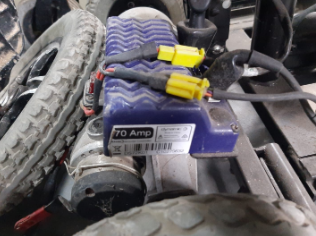
\includegraphics[width=0.75\linewidth]{Imagenes//Junio/driver.png}
\end{figure}

También se dio una entrevista en Radio Halley. Se armó el tríptico, textos para imprimir y las presentaciones para el Stand en la Técnica 3 de Solano. Se desestima el ADC 1115 para utilizar la Raspberry Pi Pico mini, ya que tiene una mayor frecuencia de switcheo. Se empieza a armar el código de la Inteligencia Artificial y se arma el código de I2C para conectar la Raspberry Pi Pico con la Pi 4. Luego se programa a la Raspberry Pi Pico para utilizar su ADC.

\begin{figure}[H]
    \centering
    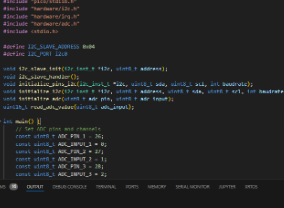
\includegraphics[width=0.6\linewidth]{Imagenes//Junio/ADC.png}
\end{figure}

\newpage

Fuimos a la muestra de la Técnica 7 de Solano y se arma el Stand. Se sigue el código de I2C y ADC.

\begin{figure}[H]
    \centering
    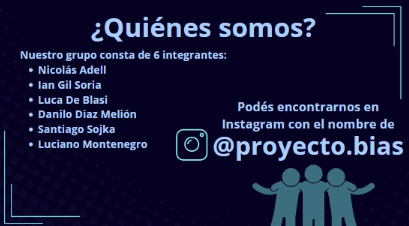
\includegraphics[width=0.6\linewidth]{Imagenes//Junio/Quienes.png}
\end{figure}

Se realiza videollamada con CILSA y se realiza nota con TV pública.

\begin{figure}[H]
    \centering
    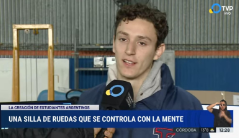
\includegraphics[width=0.5\linewidth]{Imagenes//Junio/Fabi.png}
\end{figure}

Se prueban los motores Arduino con la Raspberry Pi 4 para el sistema de emergencia.

\begin{figure}[H]
    \centering
    \includegraphics[width=0.5\linewidth]{Imagenes//Junio/Servos.png}
\end{figure}


Avances en el código para la realización de modelo de predicción. Se conectan los códigos para recepción de EEG en tiempo real. Se prueba el motor, se verifica que está quemado y se verifica la funcionalidad.

\begin{figure}[H]
    \centering
    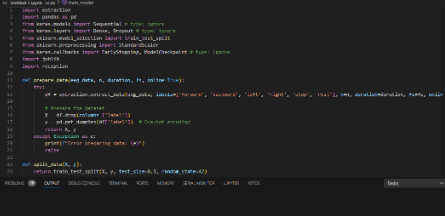
\includegraphics[width=0.65\linewidth]{Imagenes//Junio/Codigo.png}
\end{figure}


Simulación de circuito EEG y código para el filtrado digital. Se empieza a realizar la carpeta de campo. Búsqueda de puentes H y módulo PWM. Refactorización de códigos EEG. Prueba de motor.

\begin{figure}[H]
    \centering
    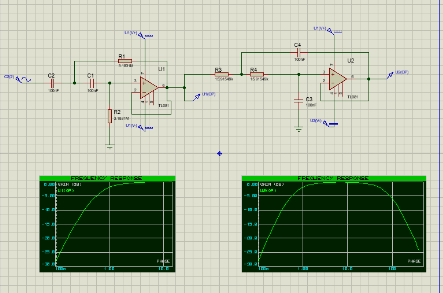
\includegraphics[width=0.5\linewidth]{Imagenes//Junio/Esquematico.png}
\end{figure}


Se soldó un potenciómetro al motor para luego probarlo. Se revisan los códigos de IA. Se saca la silla con dos motores para probarla.

\begin{figure}[H]
    \centering
    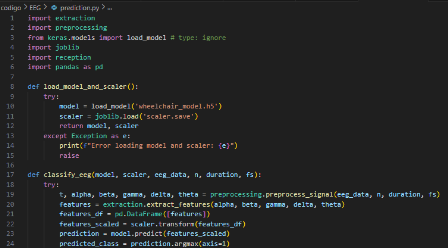
\includegraphics[width=0.75\linewidth]{Imagenes//Junio/Codigo2.png}
\end{figure}

\newpage

Se empieza a hacer funcionar al motor. El driver aun no funciona pero se detectó un código de estado del error. También se verifica el estado del freno de mano, el cual está cortocircuitado lo que produjo olor a quemado.

\begin{figure}[H]
    \centering
    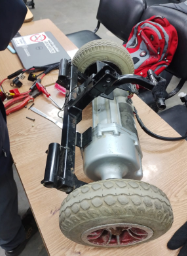
\includegraphics[width=0.5\linewidth]{Imagenes//Junio/Motor.png}
\end{figure}

Se debuggea el código de filtrado.

\begin{figure}[H]
    \centering
    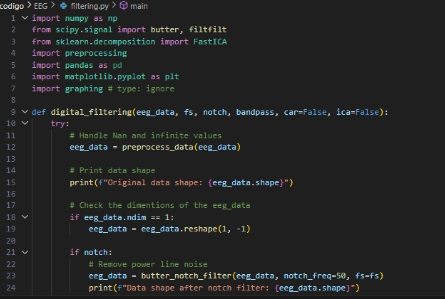
\includegraphics[width=0.75\linewidth]{Imagenes//Junio/Codigo3.png}
\end{figure}

\newpage

Avances en el debugging de extraction.py debido a inteligencia artificial utilizando datasets de la web. Descubrimos que lo más probable de hacer es realizar un dataset propio.

\begin{figure}[H]
    \centering
    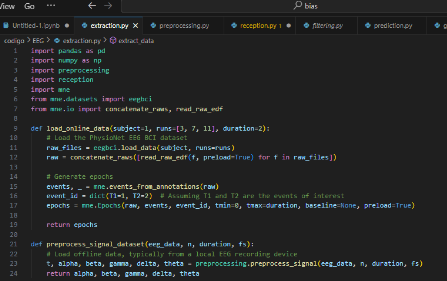
\includegraphics[width=0.75\linewidth]{Imagenes//Junio/Codigo4.png}
\end{figure}


Búsqueda de modelos de puente H. Simulación de filtrado de circuitos y rediseño de los filtros. Se empieza a realizar el diseño de KiCad. 

\begin{figure}[H]
    \centering
    \includegraphics[width=0.75\linewidth]{Imagenes//Junio/Señal.png}
\end{figure}

\newpage

Llegan algunos materiales de cooperadora y continuamos el diseño en Kicad. Se intenta probar la recepción por medio de I2C y la Raspberry Pi Pico con la Pi 4

\begin{figure}[H]
    \centering
    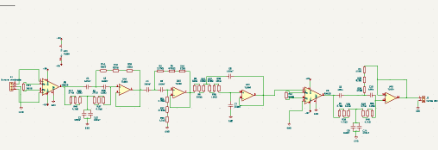
\includegraphics[width=0.95\linewidth]{Imagenes//Junio/Filtros.png}
\end{figure}


En el día de la fecha se ordenaron los materiales ordenados por cooperadora y se pidieron aquellos faltantes en el pañol y lo que no había se agregó a la lista de compra. También hicimos pruebas con los motores y logramos hacerlos funcionar, además de ponerlos en condiciones para su uso. Recibimos los electrodos del proyecto Brainstream del año pasado.

\begin{figure}[H]
    \centering
    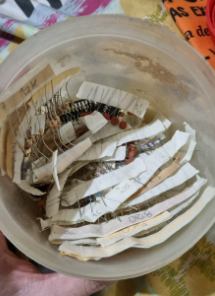
\includegraphics[width=0.45\linewidth]{Imagenes//Junio/Materiales.png}
\end{figure}



\newpage







\begin{center}
    \section{Julio de 2024}
\end{center}
Se empieza a realizar el circuito en el PCB. Se empieza a debuggear el código de recepción, aunque aún con inconvenientes en la conexión.

\begin{figure}[H]
    \centering
    \includegraphics[width=0.7\linewidth]{Imagenes//Julio/imagen_2024-10-14_135907517.png}
\end{figure}

Se encuentra un Puente H que supuestamente aguanta hasta 48 A. Se finaliza el pcb del circuito EEG. Se establece la conexión I2C entre los micros. Se prueba el circuito de filtro pasabajos. Se busca alternativa al Driver Arduino por transistores que aguanten la corriente y hacerlo por nosotros mismos. 

\begin{figure}[H]
    \centering
    \includegraphics[width=0.5\linewidth]{Imagenes//Julio/imagen_2024-10-14_140313394.png}
\end{figure}

\newpage
Se realiza la conexión I2C entre la Pi 4 y la Pi Pico. Se van refactorizando los códigos y mejorando el rendimiento de la conexión para mejorar la rapidez. Por otro lado, ya se hizo el pedido de los transistores Mosfet que soporten la corriente de 24 A para realizar el puente H.

\begin{figure}[H]
    \centering
    \includegraphics[width=0.8\linewidth]{Imagenes//Julio/imagen_2024-10-14_140420732.png}
\end{figure}
Se comenzó a realizar la carpeta técnica, tanto en word como en LaTeX. Conexión entre i2c y los microcontroladores, mejorando la velocidad para las mediciones y refactorizando el código. Creación de modelo 3D del PCB y finalización del EEG. Realización de puente H por señales PWM.

\begin{figure}[H]
    \centering
    \includegraphics[width=0.7\linewidth]{Imagenes//Julio/imagen_2024-10-14_140501734.png}
\end{figure}

\newpage
Se empieza a hacer una placa modelo para el EEG la cual luego se enviará a China para la posterior confección. Se sigue intentando con la conexión i2c, primero probándola en una Pico sola y luego la comunicación entre micros; sin embargo, siguen habiendo errores y retrasos.

\begin{figure}[H]
    \centering
    \includegraphics[width=0.5\linewidth]{Imagenes//Julio/imagen_2024-10-14_140537695.png}
\end{figure}

Se modifica el protocolo a utilizar de i2c a UART debido a una mayor simplicidad en la comunicación y menos problemas. Además, por otra parte se investigan los disipadores a utilizar en el puente H. Se confecciona finalmente el sistema de emergencia para realizar el PCB. Se descubre que se puede simular PWM por software.

\begin{figure}[H]
    \centering
    \includegraphics[width=0.8\linewidth]{Imagenes//Julio/imagen_2024-10-14_140614570.png}
\end{figure}

\newpage

\begin{center}
    \section{Agosto de 2024}
\end{center}

Se comienza a realizar el codigo para mover los motores mediante PWM. Se toma las medidas del craneo de Nicolas Fabian Adell para crear la vincha/casco para colocar los electrodos. Se soluciona el problema del refresco de las muestras. Se sigue realizando la carpeta tecnica. Se comenzo a grabar un video para reels. 

\begin{figure}[H]
    \centering
    \includegraphics[width=0.5\linewidth]{Imagenes//Agosto/imagen_2024-10-14_141352978.png}
\end{figure}

\begin{figure}[H]
    \centering
    \includegraphics[width=0.8\linewidth]{Imagenes//Agosto/imagen_2024-10-14_141408575.png}
\end{figure}

\newpage
Se empieza a corregir los otros códigos para adaptar esta nueva forma de lectura al resto de código. Se usa un template en LaTex para la documentación.

\begin{figure}[H]
    \centering
    \includegraphics[width=0.8\linewidth]{Imagenes//Agosto/imagen_2024-10-14_141439927.png}
\end{figure}

Se trabaja con los códigos de recepción y se empieza a modificar el circuito de filtro. Se sube reel a instagram. Se modifica el código para graficar.

\begin{figure}[H]
    \centering
    \includegraphics[width=0.8\linewidth]{Imagenes//Agosto/imagen_2024-10-14_141505986.png}
\end{figure}

\newpage
Se hace el código de PWM y se añaden dos filtros nuevos para el código de filtrado digital (filtro FIR y filtro IIR). Se comienza a mejorar la IA. Se mejora el pcb del puente H. Se simula circuito de offset.

\begin{figure}[H]
    \centering
    \includegraphics[width=1\linewidth]{Imagenes//Agosto/imagen_2024-10-14_141526769.png}
\end{figure}

Investigación de combinación de las señales en el EEG. Soldado de componentes placa de sistema de emergencia y filtro EEG. Se unen los códigos del Puente H y del main del sistema de emergencia. Se encuentran las formas de combinar las señales de los canales en el EEG. Se sigue realizando la carpeta técnica. Se arma el programa app.py el cual va a ser el encargado de conectar todos los códigos. En el mismo ya se implementaron la recepción constante y el procesamiento aplicado con filtros.

\begin{figure}[H]
    \centering
    \includegraphics[width=1\linewidth]{Imagenes//Agosto/imagen_2024-10-14_141539399.png}
\end{figure}

\newpage
Se decide organizar el código en programación orientada a objetos para, de esta manera, tener una mejor organización. De esta manera, se crean clases tales como DspBias, Bias, ReceptionBias y ProcessingBias, FilterBias.

\begin{figure}[H]
    \centering
    \includegraphics[width=0.8\linewidth]{Imagenes//Agosto/imagen_2024-10-14_141557883.png}
\end{figure}

Estuvimos en la feria regional de la UNQ. Se crea clase graphing y se termina diseño de la placa con la RP2040 Zero. 



Se crea la clase BiasAI para empezar a codificar. Se adapta el código para que exista un PWM invertido. Se averigua para comprar los AD620AN. Se diseña la unión de las tres partes del circuito para evitar que se filtre ruido y pueda afectar el desempeño de la Pi 4. De esta forma, se tienen dos masas distintas en todo el circuito.

\begin{figure}[H]
    \centering
    \includegraphics[width=0.7\linewidth]{Imagenes//Agosto/imagen_2024-10-14_141616815.png}
\end{figure}

Se prueban el código de los motores. Se sueldan los componentes de los circuitos de EEG y del sistema de emergencia. Se arreglan los errores del código de Emergencia.



Se termina de soldar los componentes de los circuitos. Se decide como hacer la estructura del EEG. Se sigue desarrollando la estructura de la silla. Se investiga sobre las jaulas de Faraday. Se codifica la clase BiasAI. 



Se obtiene el dinero para comprar amplificadores AD620AN. Se siguen soldando las plaquetas para luego leer señales cerebrales.

\newpage

\begin{center}
    \section{Septiembre de 2024}
\end{center}


Se trabaja con la extracción de features para el entrenamiento de la IA, utilizando señales sintetizadas. Se intenta lograr que tengan las mismas dimensiones que la capa de entrada. Se diseña el circuito de alimentaciones para la Pi 4 (etapa de control).

\begin{figure}[H]
    \centering
    \includegraphics[width=0.8\linewidth]{Imagenes//Septiembre/features.jpg}
\end{figure}

Se trabaja con los modelos de inteligencia artificial, viendo que ya se puede entrenar y va prediciendo comandos. El modelo utiliza una red neuronal convolucional.

\begin{figure}[H]
    \centering
    \includegraphics[width=1\linewidth]{Imagenes//Septiembre/prediccion.jpg}
\end{figure}

\newpage
Se sigue realizando la carpeta técnica. Se suelda el primer canal del EEG. Se investiga sobre el multiprocessing y el multithreading con python. Se realizan códigos para el multithreading. Se mide la señal de la salida de la placa de los filtros. Se prueba la corriente del motor para calcular las dimensiones de los capacitores.

\begin{figure}[H]
    \centering
    \includegraphics[width=0.5\linewidth]{Imagenes//Septiembre/multithreading.png}
\end{figure}

Probamos el circuito de filtrado y se encontró un problema. El último notch tenía las entradas inversoras y no inversoras invertidas

\begin{figure}[H]
    \centering
    \includegraphics[width=0.5\linewidth]{Imagenes//Septiembre/filtros.jpg}
\end{figure}

Probamos el circuito de filtrado y se soluciono el problema que encontramos el día anterior. Probamos el circuito de emergencia desde el PCB. Se sigue realizando la carpeta técnica. Se encuentra un error en la última etapa de notch, que por alguna razón empieza a amplificar luego de los 100 Hz.



Se avanza con el soldado de la placa de offset. A su vez se termina el diseño del puente H para imprimir y finalmente se descarga el dataset BCI IV 2a. para luego utilizarlo para el entrenamiento del modelo.

\begin{figure}[H]
    \centering
    \includegraphics[width=0.5\linewidth]{Imagenes//Septiembre/offset.jpg}
\end{figure}

Se programa un Arduino Nano 3.0 para usar un joystick y mover los motores. Por lo tanto, se crea un programa de slave para la arduino y un programa de master para la Raspberry Pi 4.

\begin{figure}[H]
    \centering
    \includegraphics[width=0.5\linewidth]{Imagenes//Septiembre/joystick.png}
\end{figure}

\newpage
Se prueba la placa de emergencia, se ve que hay un error en el buzzer y posteriormente se termina la placa de alimentación para la Pi 4. Se termina de realizar la lista para la compra de materiales. Se descubre que la plaqueta de alimentación contiene el LED rojo al revés. Se terminan de planchar las pistas del puente H y se estañan las mismas.

\begin{figure}[H]
    \centering
    \includegraphics[width=0.6\linewidth]{Imagenes//Septiembre/emergencia.png}
\end{figure}

Se prueba el circuito de offset y se descubre que el diodo Zener práctico no es igual a la simulación ya que en el mismo circula corriente aunque sea menor a la tensión esperada. Se prueba circuito de transmisión por UART y se ve que a la salida no le llega nada a la Pi 4. Se descubre que el problema en la plaqueta de la comunicación UART es la velocidad de transmisión. Se puede transmitir hasta 9600 baudios. Por esa razón, se reemplaza por un optoacoplador 6n137 y por un transistor 2n2222.

\begin{figure}[H]
    \centering
    \includegraphics[width=0.35\linewidth]{Imagenes//Septiembre/UARAT.png}
\end{figure}

Se va a hablar con una técnica neuróloga en el hospital del cruce con el objetivo de que nos muestre las instalaciones EEG y nos despeje algunas dudas de la localización de los electrodos..



Se van a comprar los componentes restantes y se resuelve el problema de la velocidad de comunicación UART mediante el reemplazo de los materiales nombrados anteriormente. Se rediseñan las placas por tema de alimentaciones y, por último, se rediseña la placa de recepción. Además, se sueldan los últimos componentes del puente H. Por otro lado, se piensa en hacer una silla de diseño 3D chiquita.


Se prueba el puente H y nos damos cuenta de un error, y es que circulan 160 A cuando ambas entradas PWM están en cero. Se prueba el circuito de filtrado en protoboard pero termina un AD620AN quemado debido a que las alimentaciones estaban invertidas. Por otro lado, se realiza la plaqueta de control de la Pi 4.

\begin{figure}[H]
    \centering
    \includegraphics[width=0.7\linewidth]{Imagenes//Septiembre/puenteh.jpg}
\end{figure}

\newpage
Se arreglan ciertas incoherencias en la “shape” del dataset del código de la IA. Se realiza el banner y se manda a cooperadora.

\begin{figure}[H]
    \centering
    \includegraphics[width=0.5\linewidth]{Imagenes/Septiembre/banner.jpg}
\end{figure}

Se prueba el circuito de filtrado sin el último filtro Notch. Este último distorsionaba la señal al punto de aumentarla hasta los 120 Hz y disminuye luego de esta frecuencia. Sin este último nos aseguramos que no haya distorsión. Se termina de soldar el circuito de control y recepción de datos. Se prueba el circuito de offset y nos damos cuenta que el zener empieza a conducir antes de que la señal se recorte, por lo que sugerimos cambiar la resistencia. De esta forma, la tensión de la resistencia será menor.

\newpage

\begin{center}
    \section{Octubre de 2024}
\end{center}

Se comienza a diseñar la jaula de Faraday. Se miden los PCBs. La silla de madera termina de ser fabricada.

\begin{figure}[H]
    \centering
    \includegraphics[width=0.75\linewidth]{Imagenes//Octubre/Faraday.jpeg}
\end{figure}

Se comienza a realizar el Informe Técnico del proyecto para presentar en las ONIET.

\begin{figure}[H]
    \centering
    \includegraphics[width=0.75\linewidth]{Imagenes//Octubre/InformeDescriptivo.jpeg}
\end{figure}

\newpage

Se probó el circuito de filtrado con los electrodos, usando la cabeza de Santiago Sojka. Se sigue realizando la carpeta técnica. Se buscan soluciones a los errores del puente H.

\begin{figure}[H]
    \centering
    \includegraphics[width=0.5\linewidth]{Imagenes/Octubre/SojkaElectrodos.png}
\end{figure}

Se prueba nuevamente la placa de filtrado con osciloscopio digital. Se prepara todo para entregar el informe descriptivo y el informe de redes sociales para las ONIET.



Se diseña un nuevo circuito de puente H que tiene más probabilidades de funcionar. Se termina y luego se refactoriza el programa que permite entrenar al algoritmo de machine learning.



Se hace funcionar el puente H con un nuevo circuito. En este caso, lo que hicimos fue hacer un cruce entre los gates de los mosfets y, de esta forma, vimos que la carga podía tener +24 V, -24 V y 0 V. Por último, se intentó probar todas las etapas de filtros y nos dimos cuenta que las baterías estaban descargadas.

\newpage

Se prueban todas las placas juntas y nos damos cuenta que hay un error en una plaqueta debido a que había una pata de resistencia haciendo cortocircuito con masa. Después, se empieza a hacer la jaula de Faraday de madera. Por último, se terminan todas las placas de filtros y se empiezan a probarlas. Se prueban todas las placas juntas para ver la gráfica de señales en la terminal con los 9 electrodos juntos.

\begin{figure}[H]
    \centering
    \includegraphics[width=0.5\linewidth]{Imagenes/Octubre/Osciloscopio.jpeg}
\end{figure}


\begin{figure}[H]
    \centering
    \includegraphics[width=0.5\linewidth]{Imagenes/Octubre/Silla.jpeg}
\end{figure}

Se termina de realizar la placa del puente H. Se empieza a diagramar las conexiones. Se avanza en realizar la carpeta técnica. Se ve que el modelo de inteligencia artificial posee un 25\% de precisión.

\begin{figure}[H]
    \centering
    \includegraphics[width=0.8\linewidth]{Imagenes//Octubre/entrenamiento model.jpg}
\end{figure}

En este día lo que se hizo fue probar el puente H con un motor de poco consumo. Se prueba el modelo con SVM y CSP para ver cómo se comportan antes las señales. Se modifican las dimensiones de las señales y de las features para poder entrenarlas.



Lo que se prueba en este día es la utilización del filtrado PCA para ver el comportamiento de la IA.


\newpage










\end{document}
